\section{Results and Discussion}

Some behavioural traits are shared and persist within communities due to social learning \parencite{viciana2021}. We refer to these behaviours as 'animal culture', exemplified by tool use in capuchin monkeys \parencite{falotico2019}, the learned songs of oscine birds, migration routes \parencite{jesmer2018, berdahl2018, byholm2022}, and the feeding techniques of some cetaceans \parencite{allen2013, rendell2001}. Animal cultures are not static: neutral and selective mechanisms influence the frequency of cultural traits \parencite{potvin2015, williams2021}, leading to a process of cultural evolution. The resulting cultural traditions vastly differ in their diversity and stability \parencite{tchernichovski2017}, determined by both learning biases and mechanisms and the demographic structure of populations \parencite{deffner2022a, kandler2017}. 

While the role of social learning strategies and biases---frequency dependence, tutor biases, etc.---has been extensively studied \parencite{pike2010, kendal2015, aplin2017, lachlan2018, tchernichovski2021}, there exists a substantial gap in our understanding of how demography contributes to the emergence and persistence of distinct cultural traits within wild populations. Processes such as the recruitment of juveniles and immigrants, emigration, mortality, and variation in age structure are likely to strongly affect an individual's opportunities for learning and exposure to different cultural variants, which has been amply emphasized by theoretical work \parencite{deffner2022a, deffner2022, kandler2023, fogarty2019, deffner2020, derex2016, kirby2021, nunn2009, barta2023}. Despite this, translating theoretical expectations into empirical evidence remains a challenge. (See \cite{chimento2021, fayet2014} for exceptions). 


\begin{figure*}[hbt!]
    \centering
    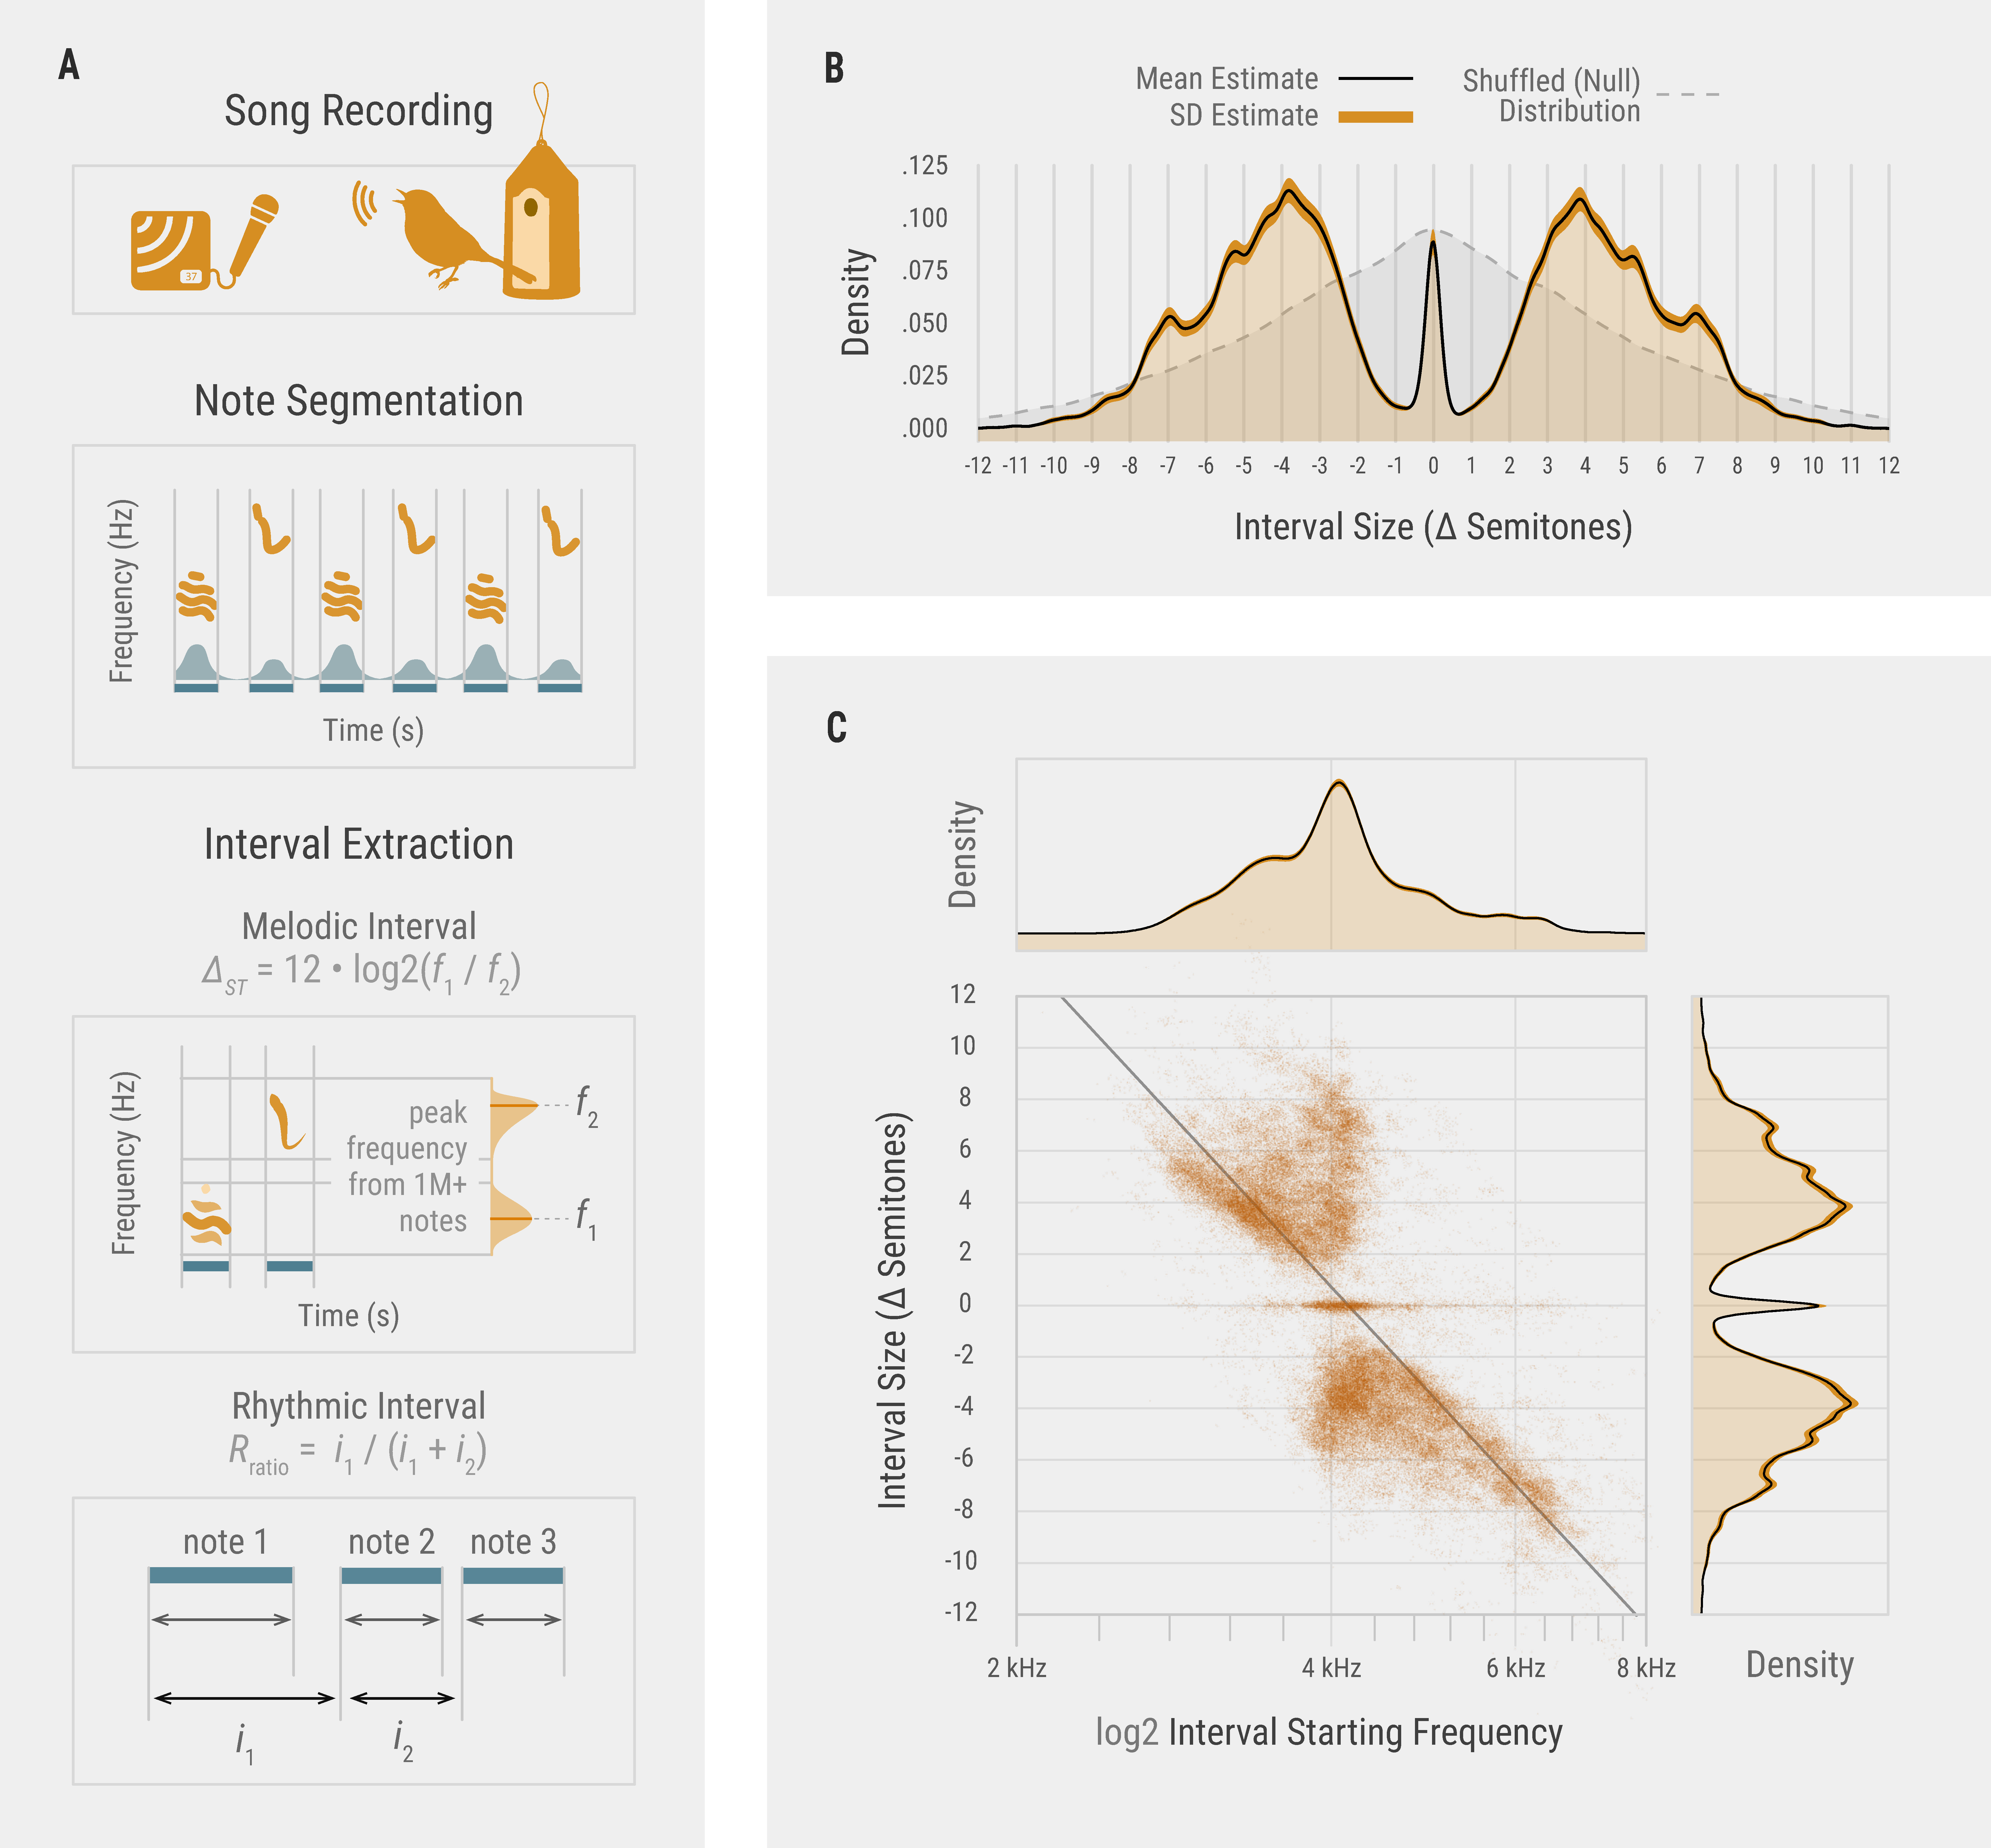
\includegraphics[width=\linewidth]{figures/chapter_5/methods-melodic-null.pdf}
    \mycaption{Visual description of the methods; melodic structure in great tit songs}{
        (A) Cultural variables measured at the neighbourhood level. See methods for definitions.
        (B) Variation in the properties and composition of neighbourhoods across the population. See methods for definitions.
        (C) 3D render of our study site, Wytham Woods, based on first return LiDAR data \parencite{defra2020}. Elevation is exaggerated. The network represents pairwise song cultural distances between individuals with known spatial locations, used in the models reported in Fig. 2. Aquamarine (darker) arrows represent natal dispersal within the population, and the yellow (lighter) arrow represents immigration into the population, two of the variables used in this work. Age and bird (individual) turnover are not depicted.        
    }
    \label{c5_fig:methods}
\end{figure*}




\begin{figure*}[th!]
    \centering
    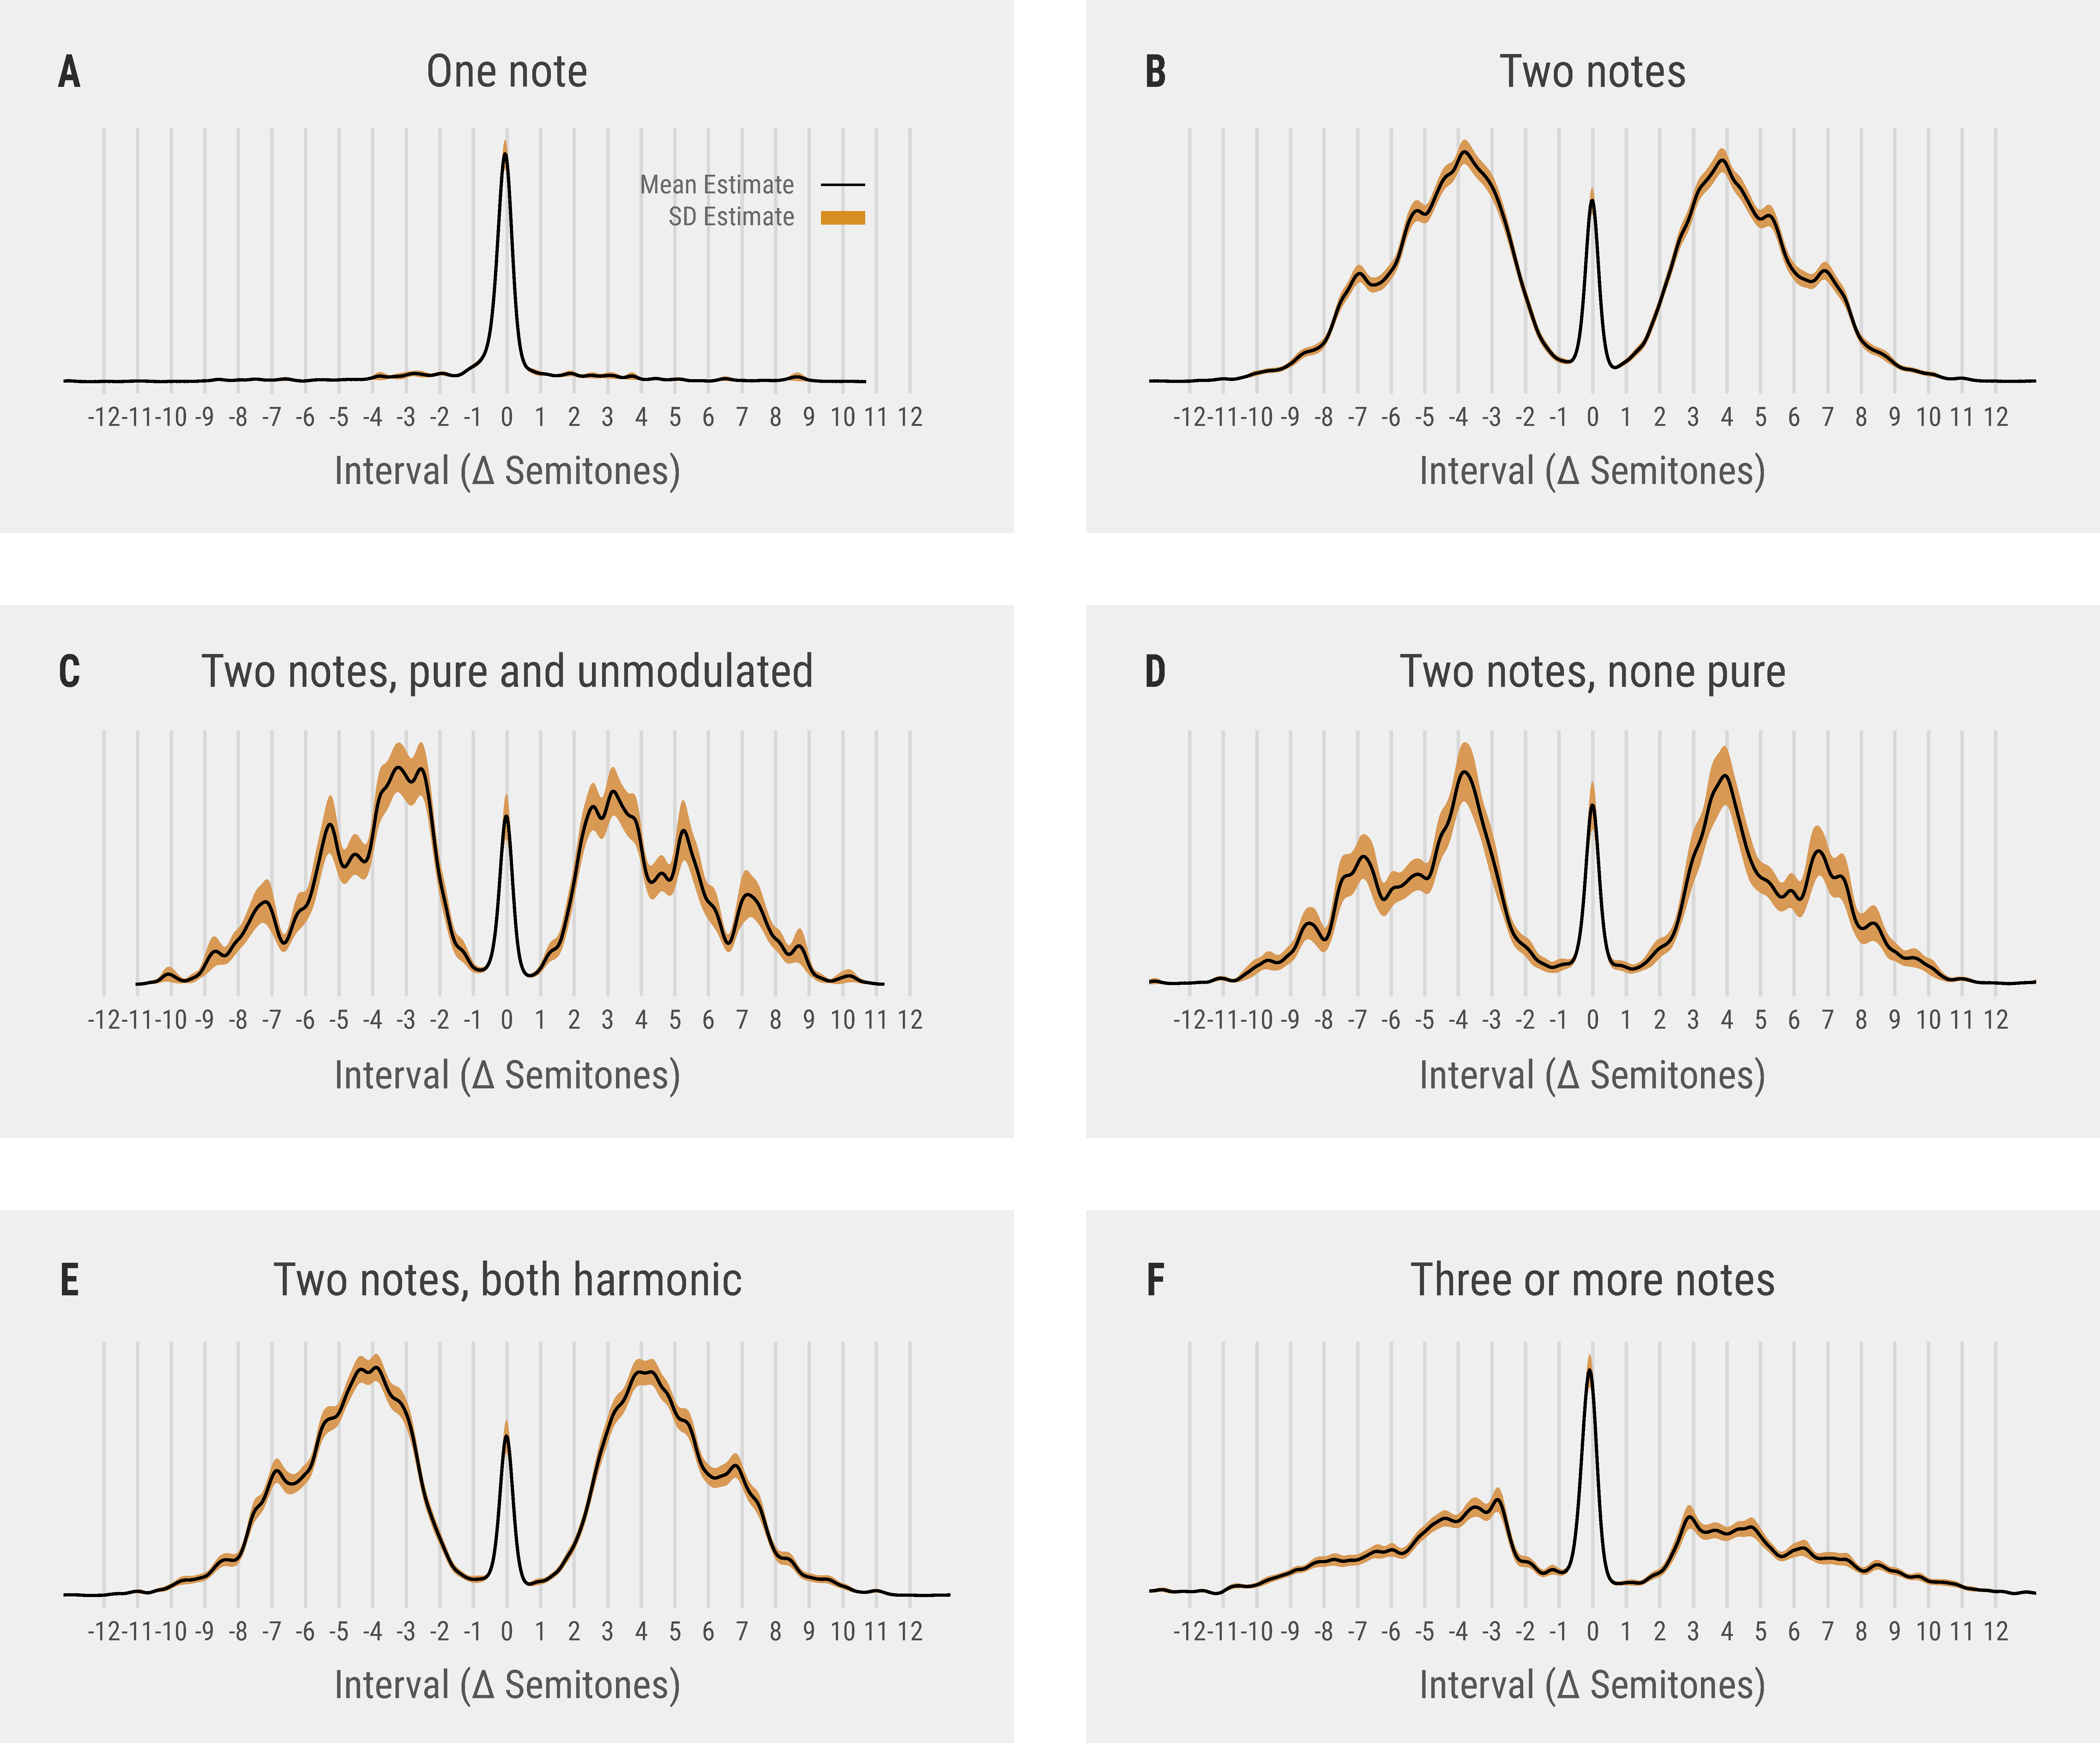
\includegraphics[width=\linewidth]{figures/chapter_5/melodic-songtypes.pdf}
    \mycaption{Density estimate of the distribution of melodic intervals across a typology of songs}{
        (A) Marginal effects at the mean of neighbourhood characteristics including mean dispersal distance, proportion of immigrant birds, average age, and individual turnover.
        (B) Adjusted predictions and partial residuals of the effect of mean dispersal distance on cultural novelty. Low-dispersal neighbourhoods are those in which birds were born in the same area.
        (C) Adjusted predictions and partial residuals of the effect of the mean age of the neighbourhood on cultural diversity. A neighbourhood with a mean age of 1 would be one where all birds are breeding for the first time.
        (D) The average distribution of cultural diversity in the population across space during the study period (2020-2022). This map captures the residual variation in cultural diversity after taking into account the demographic variables in (A). The map is based on a Gaussian process model with an exponentiated-quadratic kernel covariance function, which allows us to interpolate between the locations where we have data.
    }
    \label{c5_fig:melodic-songtypes}
\end{figure*}


\begin{figure*}[b]
    \centering
    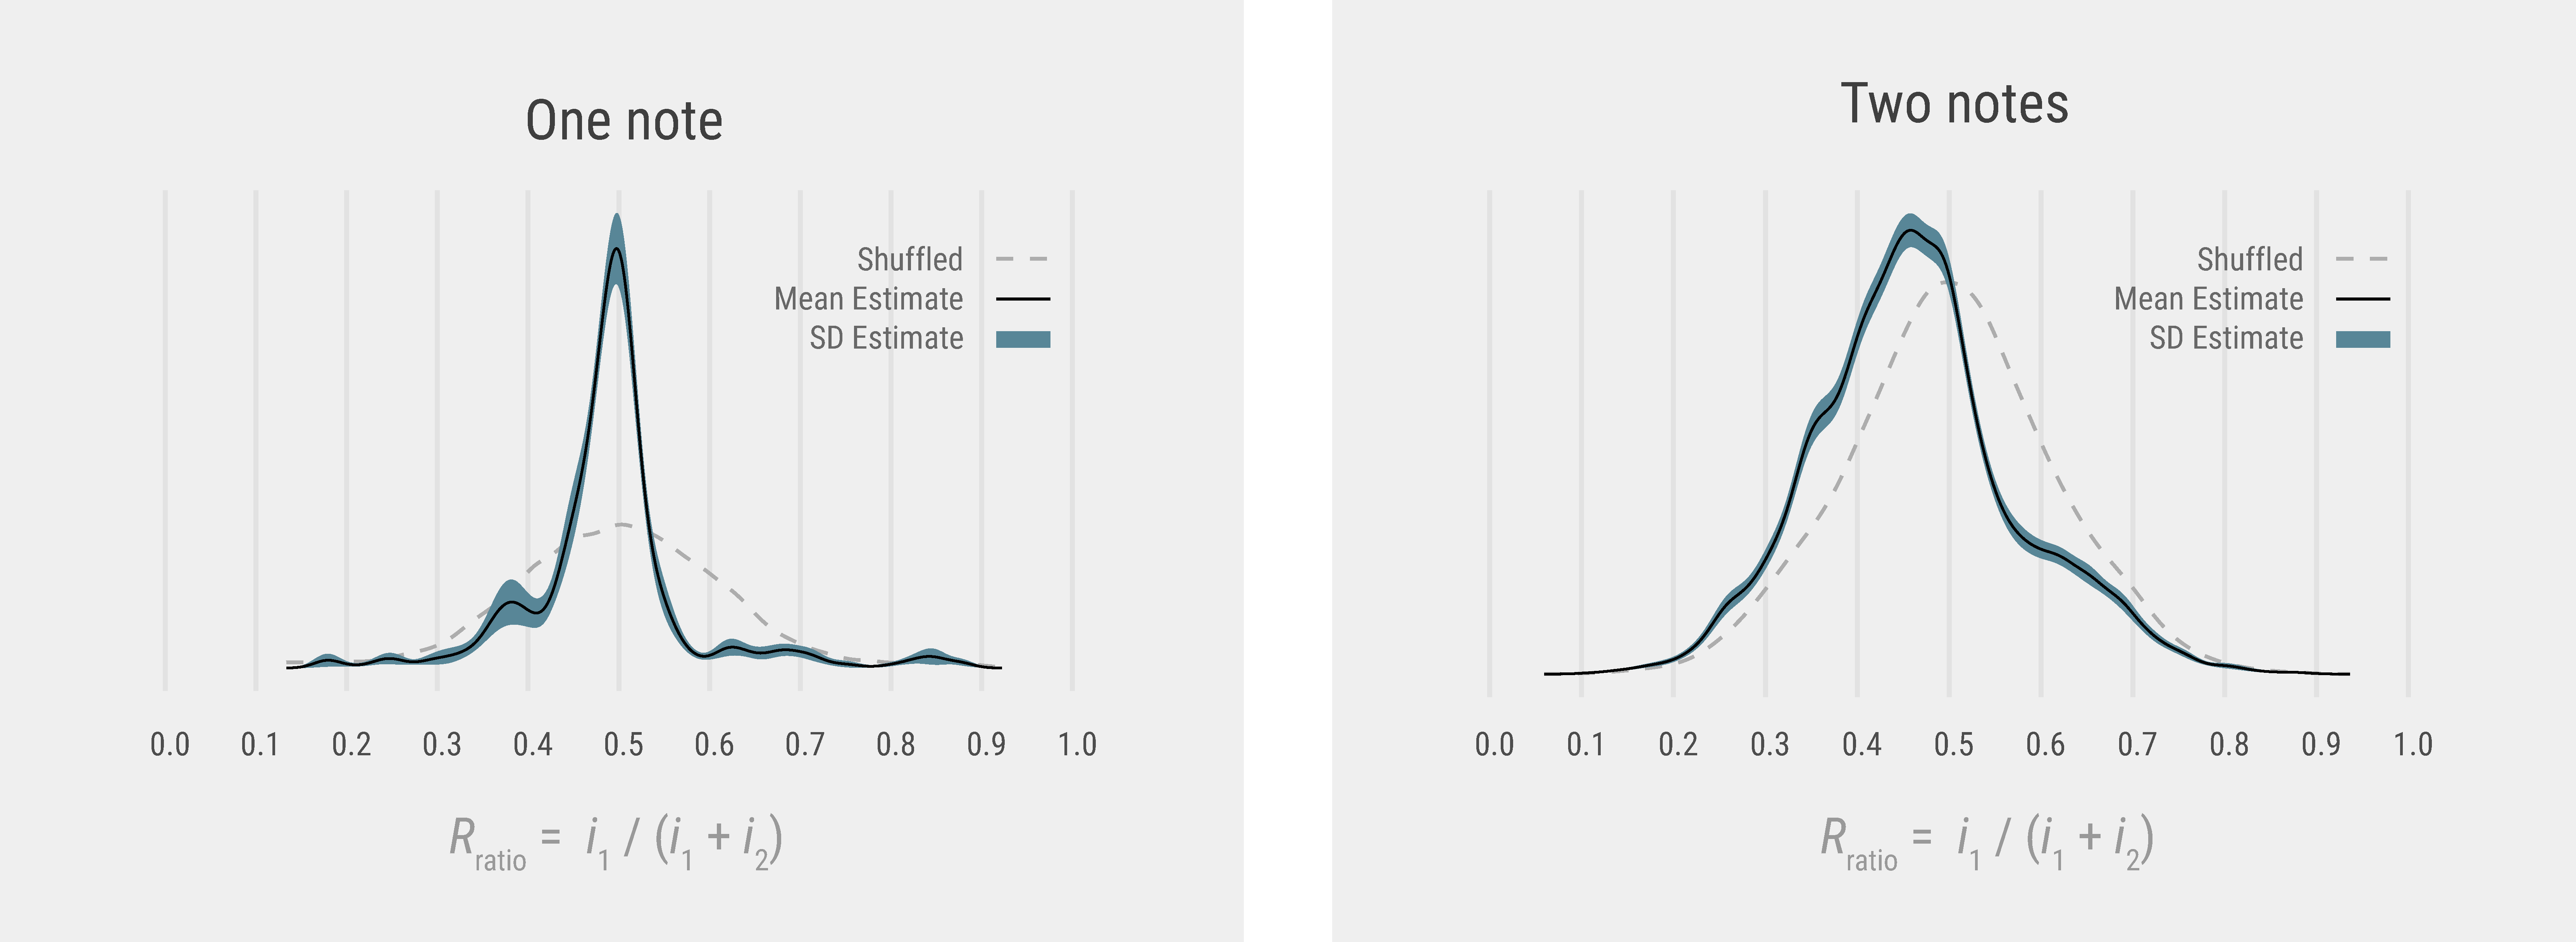
\includegraphics[width=\linewidth]{figures/chapter_5/rhythmic-nulls.pdf}
    \mycaption{Rhythmic patterns in one and two-note songs}{
        (A) Illustrative example showing the repertoires of two different birds in the population, with three songs in each, one of which is shared. Each sub-panel shows a stylized spectrogram, with time in the horizontal axis and frequency in the vertical. Units not shown.
        (C) Marginal effects (ME) of dispersal, immigration status, and age on song repertoire similarity between individuals. Dispersal: Birds that are close neighbours are more culturally similar, regardless of where they were born, whereas natal distance may have a weak positive effect on cultural similarity. Immigration: There is no strong evidence that birds born outside the population are dissimilar from resident birds. Age difference: Birds are less culturally similar the greater the difference in their birth years.
    }
    \label{c5_fig:rhythmic-nulls}
\end{figure*}


\section{Acknowledgements}

We thank all those who have contributed to the long-term nest box study in Wytham Woods and the collection of associated data. This work was supported by a Clarendon-Mary Frances Wagley Graduate Scholarship and an EGI scholarship to Nilo Merino Recalde, and made use of the University of Oxford Advanced Research Computing facility \parencite{richards2015}.

\section{Author contributions}
\textbf{Nilo Merino Recalde}: Conceptualization, Methodology, Software, Formal analysis, Investigation, Data Curation, Writing - Original Draft, Writing - Review \& Editing, Visualization. 
\textbf{Andrea Estandía}: Investigation, Data Curation, Writing - Review \& Editing.
\textbf{Ella F. Cole}: Supervision, Project administration, Writing – review and editing.
\textbf{Ben C. Sheldon}: Supervision, Project administration, Writing – review and editing, Funding acquisition.

\renewcommand{\cleardoublepage}{}
\renewcommand{\clearpage}{}
\printbibliography
